\documentclass[journal,12pt,onecolumn]{IEEEtran}
\usepackage{graphicx, float}
\graphicspath{{Figs/}}
\usepackage{multicol}
\usepackage{parskip}
\usepackage{titlesec}
\usepackage{color}
\usepackage{enumitem}
\usepackage{amsmath,amssymb,amsfonts,amsthm}
\usepackage{array}
\usepackage{booktabs}
\usepackage[table]{xcolor}
\usepackage{longtable}
\usepackage{gensymb}
\usepackage{cite}
\usepackage{algorithmic}
\usepackage{textcomp}
\usepackage{txfonts}
\usepackage{listings}
\usepackage{mathtools}
\usepackage{comment}
\usepackage{tkz-euclide}
\usepackage[breaklinks=true]{hyperref}
\usepackage{gvv}
\usepackage[latin1]{inputenc}
\usetikzlibrary{arrows.meta, positioning}
\usepackage{xparse}
\usepackage{calc}
\usepackage{multirow}
\usepackage{hhline}
\usepackage{ifthen}
\usepackage{lscape}
\usepackage{tabularx}
\usepackage{circuitikz}
\usepackage{tikz}
\newtheorem{problem}{Problem}
\newtheorem{theorem}{Theorem}[section]
\newtheorem{proposition}{Proposition}[section]
\newtheorem{lemma}{Lemma}[section]
\newtheorem{corollary}[theorem]{Corollary}
\newtheorem{example}{Example}[section]
\newtheorem{definition}[problem]{Definition}
\newcommand{\BEQA}{\begin{eqnarray}}
\newcommand{\EEQA}{\end{eqnarray}}
\theoremstyle{remark}
\title{Graduate Aptitude Test in Engineering 2017}
\author{EE25BTECH11025- Vishwambhar}

\begin{document}

\maketitle

\begin{enumerate}
 
\item If a vector $\vec{v}$ has components $v_x = 1$, $v_y = 2$,$v_z = 3$, then its magnitude is \dots.\\
(write answer with two decimal places)\\

\hfill{(GATE PE 2017)}

\item The value of $\lim\limits_{x \to 0} \frac{(2 + x)^4 - 16}{x} $ is \dots.\\

\hfill{(GATE PE 2017)}

\item If $\frac{d^2 y}{dx^2} + f\brak{x, y} = 0$ is to be solved using the conditions $y(0) = a$ and $y(1) = b$, which of the following numerical method(s) can be used?
\begin{enumerate}
\item Euler with shooting method
\item Euler without shooting method
\item 4th order Runge-Kutta with shooting method
\item Both (A) and (C)
\end{enumerate}
\hfill{(GATE PE 2017)}

\item The numerical method used to find the root of a non-linear algebraic equation, that converges quadratically, is:
\begin{enumerate}
\item Bisection method.
\item Regula-falsi method (Method of False Position).
\item Newton-Raphson method.
\item None of above.
\end{enumerate}
\hfill{(GATE PE 2017)}

\item Which one of the following curves shows a typical behavior of the producing gas oil ratio (GOR) with time for a reservoir under solution gas drive?
\begin{figure}[h]
    \centering
    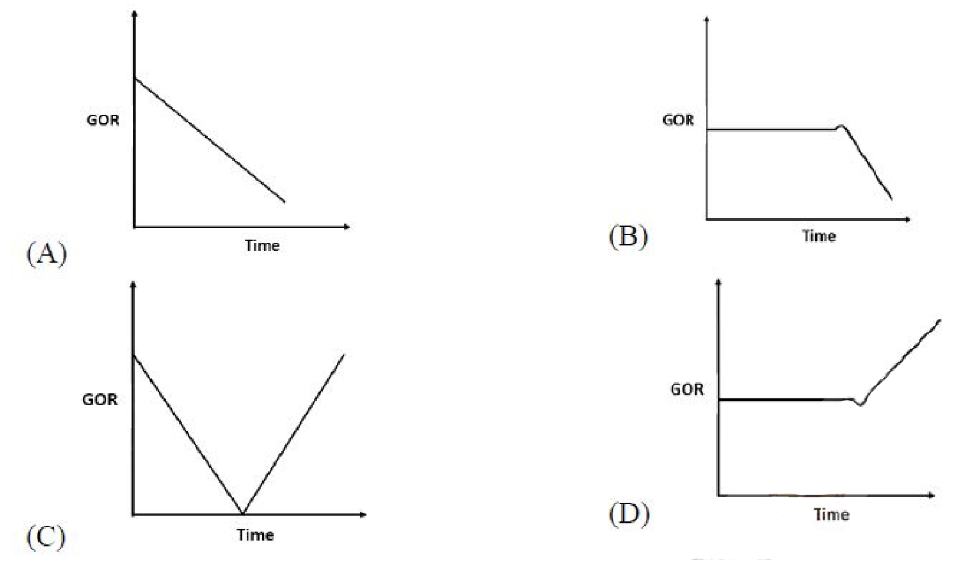
\includegraphics[width=0.5\columnwidth]{GraphQ _5.png}
    \caption{}
    \label{fig:placeholder}
\end{figure}
\hfill{(GATE PE 2017)}

\item A student has written the following possible causes of lost circulation during a drilling operation:
\begin{enumerate}
\item High salinity in the reservoir \\
\item Fracture in the reservoir \\
\item A fault encountered during drilling \\
\item Low viscosity of the reservoir fluid
\end{enumerate}

Which of the above statements are correct?
\begin{enumerate}
\begin{multicols}{4}
\item i, iv
\item ii, iii
\item i, iii
\item ii, iv
\end{multicols}
\end{enumerate}
\hfill{(GATE PE 2017)}

\item For water depth less than 8 m, which one of the following drilling vessels is the most suitable and economical?
\begin{enumerate}
    \item Semi-submersible rig
    \item Jack-up rig
    \item Drilling barges
    \item Drill ship
\end{enumerate}
\hfill{(GATE PE 2017)}

\item Which one of the following statements is correct for pseudo-steady state condition in a confined reservoir?
\begin{enumerate}
\item The pressure decline stops in the reservoir.
\item The pressure declines at the same rate across the reservoir.
\item The boundary pressure does not change.
\item The pressure starts increasing in the reservoir.
\end{enumerate}
\hfill{(GATE PE 2017)}

\item The roots of the equation $ \frac{d^3 y}{dx^3} - 6 \frac{d^2 y}{dx^2} + 11 \frac{dy}{dx} - 6y = 0$ are:
\begin{enumerate}
\begin{multicols}{4}
\item 1,1,2
\item 1,2,3
\item 1,3,4
\item 1,2,4
\end{multicols}
\end{enumerate}
\hfill{(GATE PE 2017)}

\item The API of a crude oil of density $950\, \text {kg/m}^3$ is \dots. (write answer with two decimal places)\\

\hfill{(GATE PE 2017)}

\item The differential equation $2xy \, dx + \brak{1 + x^2} \, dy = 0,$in which $x$ is an independent variable and $y$ is the dependent variable, is:
\begin{enumerate}
\item an ordinary differential equation of second order.
\item a first order nonlinear differential equation.
\item an exact differential equation.
\item a partial differential equation.
\end{enumerate}
\hfill{(GATE PE 2017)}

\item For the two matrices $X=
\myvec{
1 & 2 & 3\\
4 & 5 & 6
}$ $Y=
\myvec{
7 & 0\\
8 & -1
}$ the product $YX$ will be:
\begin{enumerate}
\item $XY = \myvec{ 
50 & 4 \\ 
122 & 13 
}$
\item $XY = \myvec{ 
4 & 11 & 18 \\ 
7 & 14 & 21 
}$
\item $XY = \myvec{ 
7 & 14 & 21 \\ 
4 & 11 & 18 
}$
\item $XY =\myvec{ 
18 & 5 & 6 \\ 
7 & 14 & 21 
}$
\end{enumerate}
\hfill{(GATE PE 2017)}

\item As per the Bharat IV norms, the maximum permissible limit of sulfur in diesel in ppm is:
\begin{enumerate}
\begin{multicols}{4}
\item 10
\item 50
\item 100
\item 500
\end{multicols}
\end{enumerate}
\hfill{(GATE PE 2017)}

\item The amount of methane gas evolved at $0\degree C$ and 1 atm from the dissociation of 1 m$^3$ of methane gas hydrate, is approximately:
\begin{enumerate}
\item equal to the volume of gas hydrate.
\item 10 times the volume of gas hydrate.
\item 160 times the volume of gas hydrates.
\item 300 times the volume of gas hydrates.
\end{enumerate}
\hfill{(GATE PE 2017)}

\item For a centrifugal pump, the head developed by the pump is proportional to the:
\begin{enumerate}
\item speed of the impeller rotation.
\item square of speed of the impeller rotation.
\item cubic power of speed of the impeller rotation.
\item square root of speed of the impeller rotation.
\end{enumerate}
\hfill{(GATE PE 2017)}

\item Which of these is a must for petroleum generation and accumulation?
\begin{enumerate}
\item Source rocks
\item Porous reservoir rocks
\item Impermeable cap rocks
\item All of the above
\end{enumerate}
\hfill{(GATE PE 2017)}

\item The problem of viscous fingering is encountered when:
\begin{enumerate}
\item a low viscosity fluid is injected in a high viscosity fluid.
\item a high viscosity fluid is injected in a low viscosity fluid.
\item a fluid of equal viscosity but lower density is injected in a fluid of higher density.
\item none of the above.
\end{enumerate}
\hfill{(GATE PE 2017)}

\item Which of these is \textbf{NOT} a sedimentary rock?
\begin{enumerate}
\item Shale
\item Sandstone
\item Carbonate
\item None of the above
\end{enumerate}
\hfill{(GATE PE 2017)}

\item The \textbf{unbiased} sample variance for the set of numbers: $S = \{40, 45, 50, 55, 60\}$ is \dots. (write answer with one decimal place)\\

\hfill{(GATE PE 2017)}

\item If $ 5x + 2iy - ix + 7y = 2 + 3i,$ where $i = \sqrt{-1}$, the values of two real numbers $\brak{x, y}$ are, respectively:
\begin{enumerate}
\begin{multicols}{4}
\item (-1,1)
\item (1,-1)
\item (1,1)
\item (-1,-1)
\end{multicols}
\end{enumerate}
\hfill{(GATE PE 2017)}

\item Pick the \textbf{INCORRECT} inequality, where $z_1$, $z_2$, and $z_3$ are complex numbers.
\begin{enumerate}
\item $|z_1 + z_2| \leq |z_1| + |z_2|$
\item $|z_1 - z_2| \geq |\,|z_1| - |z_2|\,|$
\item $|z_1 - z_2| \leq |z_1| - |z_2|$
\item $|z_1 + z_2 + z_3| \leq |z_1| + |z_2| + |z_3|$
\end{enumerate}
\hfill{(GATE PE 2017)}

\item Which of the following is \textbf{NOT} true? ($i = \sqrt{-1}$)
\begin{enumerate}
\item $\cos \theta = \dfrac{e^{i\theta} + e^{-i\theta}}{2}$
\item $e^{i\theta} = \cos \theta + i \sin \theta$
\item $\sin \theta = \dfrac{e^{i\theta} - e^{-i\theta}}{2i}$
\item $\cos \theta = \dfrac{e^{i\theta} + e^{-i\theta}}{2i}$
\end{enumerate}
\hfill{(GATE PE 2017)}

\item Which of the following is a potential environmental threat due to the cement-plug deterioration in an abandoned oil well?
\begin{enumerate}
\item Well bore could leak oil reservoir fluids into groundwater
\item Oil reservoir fluids could flow to the surface and contaminate surface soil
\item Oil reservoir fluids could discharge into navigable waters
\item All of the above
\end{enumerate}
\hfill{(GATE PE 2017)}

\item \dots is a mode of flame propagation in a pre-mixed gas, and drives a leading shock front into the quiescent, unburnt gas at supersonic velocity, immediately followed by a combustion zone.
\begin{enumerate}
\item Deflagration
\item Fire
\item Detonation
\item Ignition
\end{enumerate}
\hfill{(GATE PE 2017)}

\item Bio-Gas (BG), Coal Bed Methane (CBM), and Methane Gas Hydrate (MGH), if arranged in the order of increasing methane content, the correct order is:
\begin{enumerate}
\item BG, CBM, MGH
\item CBM, BG, MGH
\item CBM, MGH, BG
\item BG, MGH, CBM
\end{enumerate}
\hfill{(GATE PE 2017)}

\item For a velocity field given by $\vec{v} = y \hat{i} - x \hat{j} + 0 \hat{k}$, calculate the curl of $\vec{v}$. If the calculated vector is $a \hat{i} + b \hat{j} + c \hat{k}$, then the value of $c$ is \dots.\\

\hfill{(GATE PE 2017)}

\item Single step integration (step size = 0.5) of $ I = \int_0^1 x^2 e^x \, dx,$evaluated \textbf{numerically} using the Simpson's 1/3 rule, is \dots. (write answer with three decimal places)\\

\hfill{(GATE PE 2017)}

\item Solve $ \frac{dy}{dx} = -y$ \textbf{numerically} from $x = 0$ to $1$ using explicit, forward, first order Euler method with initial condition of $y(0) = 1$ and step size ($h$) of 0.2. The absolute value of error in $y(1)$ calculated using analytical and numerical solution is \dots \% (calculate the error using analytical solution as the basis and use three decimal places).\\

\hfill{(GATE PE 2017)}

\item Relative permeability curves are shown in the following figure for a water-oil system in a porous medium. $S_w$ is water saturation and $k_r$ is relative permeability. Curve 1 is relative permeability of water and Curve 2 is relative permeability of oil.
Assuming the porous medium is at irreducible water saturation initially, the maximum possible recovery of oil by water flooding is \dots \%. (write answer with one decimal place)\\

\hfill{(GATE PE 2017)}
\begin{figure}[h]
    \centering
    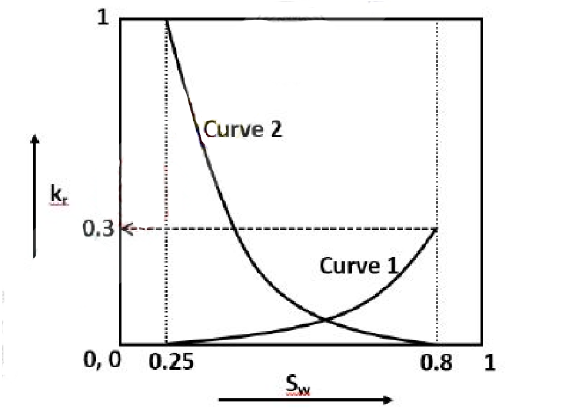
\includegraphics[width=0.5\columnwidth]{GraphQ_29.png}
    \caption{}
    \label{fig:placeholder}
\end{figure}

\item An oil reservoir of $1000$ m$^2$ area and thickness of $10$ m has a porosity of 30\%. The connate water saturation is 20\%. Initial formation volume factor $B_o = 1.2 \dfrac{\text{reservoir m}^3}{\text{stock tank m}^3}$. Assuming average oil flow rate of 2 m$^3$/day (at surface condition), the life of reservoir is \dots days.\\

\hfill{(GATE PE 2017)}

\item A self-flowing production well of depth 3,000 m having oil with density 850 kg/m$^3$ is shut-in for workover job. The shut-in pressure at the surface is $70 \times 10^5$ N/m$^2$. The density of the mud required to kill the well will be \dots kg/m$^3$. ($g = 9.81$ m/s$^2$, write answer with one decimal place)\\

\hfill{(GATE PE 2017)}

\item In a directional well, the kick off point has a true vertical depth (TVD) of 1000 m and the end of buildup section has a TVD of 1200 m. The buildup section for directional drilling has a horizontal displacement of 200 m, after which the tangent section has inclination of 45\degree.
A driller monitors the well from the surface location of the well and sees that the target has horizontal departure of 1000 m. The TVD of the deepest point of the well is \dots meters.\\

\hfill{(GATE PE 2017)}

\item The figure below shows the pressure measured in a well at different depths. AB is gas cap, B is gas-oil contact and C is water-oil contact. Density of gas in gas cap is 2 kg/m$^3$, oil density is 800 kg/m$^3$ and water density is 1000 kg/m$^3$.
The difference between pressure at point D and point B {$\brak{P_D - P_B}$ is \dots $\times 10^5$ N/m$^2$. (use $g = 9.81$ m/s$^2$, write answer with one decimal place)\\
\begin{figure}[h]
    \centering
    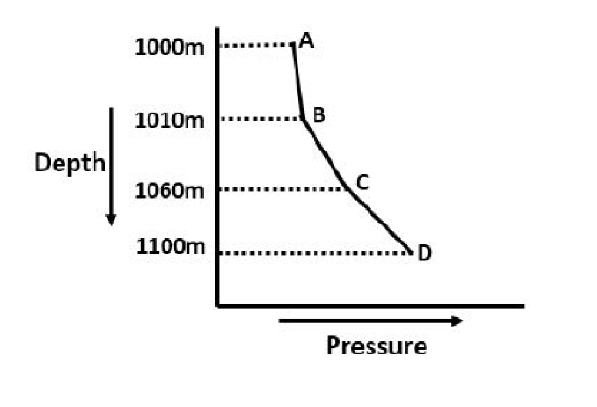
\includegraphics[width=0.5\columnwidth]{GraphQ _33.png}
    \caption{}
    \label{fig:placeholder}
\end{figure}
\hfill{(GATE PE 2017)}
\item A laboratory air-brine capillary pressure of $1.20 \times 10^5$ N/m$^2$ has been measured in a reservoir core sample at residual water saturation. The air-brine surface tension is 0.070 N/m, and the brine-oil interfacial tension for the reservoir fluid is 0.025 N/m. The density values of brine and oil are 1080 kg/m$^3$ and 780 kg/m$^3$, respectively.
Take $g = 9.81$ m/s$^2$, and assume identical wetting preferences for the core sample and reservoir. The height of the water-oil transition zone (up to the point of reservoir where connate water saturation is reached) from the free water level is \dots meters. (write answer with two decimal places)\\

\hfill{(GATE PE 2017)}

\item The eigenvalues for the matrix $ \myvec{
1 & 3 \\
4 & 2 
}$ are:
\begin{enumerate}
\item 2 and 5
\item -2 and -5
\item -2 and 5
\item none of the above
\end{enumerate}
\hfill{(GATE PE 2017)}

\item The temperature time profile for a system is given as follows:
$ \frac{dT}{dt} + 5T = 500,$ where $T$ is temperature in °C, and $t$ is time in hours. The initial condition is $T(0) = 500\degree$C.
The temperature of the system after 1 hour is \dots °C. (write answer with two decimal places)\\

\hfill{(GATE PE 2017)}

\item A porous medium is blended with three types of sediment fractions: fine pebble gravel with porosity ($\phi_{pebble} = 38\%$), sand ($\phi_{sand} = 32\%$) and fine sand ($\phi_{fine\_sand} = 30\%$). The three sediments are mixed in such proportions that the sand fills the pore volume of fine pebbles completely, and the fine sand fills the pore volume of sand completely.
The total porosity of such an irregular system is \dots \%. (write answer with two decimal places)\\

\hfill{(GATE PE 2017)}

\item Match the following:\\
\begin{enumerate}
    \item (P) Sandstone  (I)Clastic rocks\\
    \item (Q) Limestone (II)Nonclastic rocks\\
    \item (R) Shale
    \item (S) Gypsum
\end{enumerate}
\begin{enumerate}
    \item P-I, Q-I, R-II, S-II
    \item P-II, Q-I, R-I, S-I
    \item P-I, Q-II, R-I, S-II
    \item P-II, Q-I, R-II, S-I
\end{enumerate}
\hfill{(GATE PE 2017)}

\item Oil of density 900 kg/m$^3$ is flowing at 100 m$^3$/day through a horizontal pipeline having a diameter reduction from 0.1 m to 0.05 m as shown in the following figure.
The kinetic energy pressure drop ($P_1 - P_2$) caused by the diameter change is \dots N/m$^2$.
(Assume frictional losses to be negligible, write answer with one decimal place)\\
\begin{figure}[h]
    \centering
    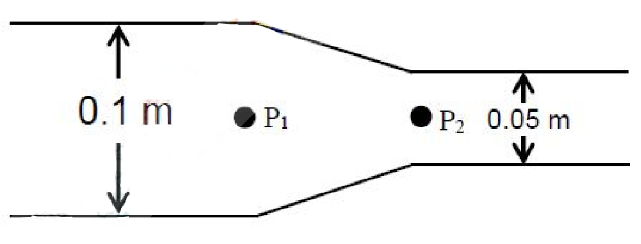
\includegraphics[width=0.5\columnwidth]{figQ_39.png}
    \caption{}
    \label{fig:placeholder}
\end{figure}
\hfill{(GATE PE 2017)}

\item Match the following EOR techniques and the principle behind them:\\

\begin{tabular}{ll}
(P) Surfactant flooding & (I) Lower the viscosity of the oil phase \\
(Q) Polymer flooding & (II) Increase the viscosity of the aqueous phase \\
(R) Steam flooding & (III) Lower the oil-water interfacial tension \\
(S) Sea water flooding & (IV) Influence the wettability of the rock \\
\end{tabular}
\begin{enumerate}
\item P-I, Q-II, R-III, S-IV \\
\item P-III, Q-II, R-IV, S-I \\
\item P-III, Q-II, R-I, S-IV \\
\item P-III, Q-I, R-II, S-IV
\end{enumerate}
\hfill{(GATE PE 2017)}

\item The viscosity-shear rate curve for a fluid is shown in the following plot. Which one of the following options best describes the behavior of the fluid in the regions I, II, and III, respectively?

\begin{enumerate}
\item Newtonian, Shear thinning, Shear thickening
\item Shear thinning, Newtonian, Shear thickening
\item Shear thickening, Newtonian, Shear thinning
\item Shear thinning, Shear thickening, Newtonian
\end{enumerate}
\hfill{(GATE PE 2017)}
\begin{figure}[h]
    \centering
    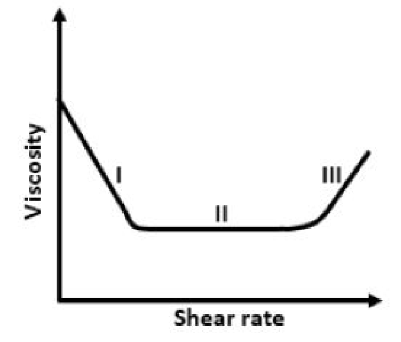
\includegraphics[width=0.5\columnwidth]{Graph_Q41.png}
    \caption{}
    \label{fig:placeholder}
\end{figure}
\item The value of constant $a$ for which:$ f(x) = \begin{cases}ax^2, & 0 \leq x \leq 5 \\0, & \text{otherwise}
\end{cases}$is a valid probability density function, is (given, $a \geq 0$):
\begin{enumerate}
\begin{multicols}{4}
\item $\dfrac{1}{125}$
\item $\dfrac{3}{125}$
\item $\dfrac{6}{125}$
\item $\dfrac{9}{125}$
\end{multicols}
\end{enumerate}
\hfill{(GATE PE 2017)}

\item $z = \frac{3^{30} - i^{19}}{2i - 1}, \quad \text{where } i = \sqrt{-1},$ would simplify to:
\begin{enumerate}
\begin{multicols}{4}
\item $1 - i$
\item $1$
\item $-i$
\item $1 + i$
\end{multicols}
\end{enumerate}
\hfill{(GATE PE 2017)}

\item A well of radius 0.25 m is drilled. Mud invasion in the formation caused a skin radius of 2 m and reduced the permeability of the damaged zone to 30 mD. Well test revealed that the skin factor of the damaged zone is 2.3.
The permeability of the unaffected formation will be \dots mD. (write answer with one decimal place)\\

\hfill{(GATE PE 2017)}

\item The average reservoir pressure and fracture gradient of petroleum formation at a depth of 4,000 m are 30,000 kN/m$^2$ and 16 (kN/m$^2$)/m, respectively.
The density of the formation is 2290 kg/m$^3$. If the reservoir pressure declines to 20,000 kN/m$^2$ after a few years of production, the fracture gradient of the formation is \dots(kN/m$^2$)/m. (write answer with one decimal place)\\

\hfill{(GATE PE 2017)}

\item Match the following:\\

\begin{tabular}{ll}
(P) Gamma ray log & (I) Water saturation \\
(Q) Resistivity log & (II) Acoustic waves \\
(R) Cement bond log & (III) Permeability \\
(S) NMR log & (IV) Lithology \\
\end{tabular}
\begin{enumerate}
\item P-IV, Q-I, R-II, S-III \\
\item P-I, Q-II, R-III, S-IV \\
\item P-I, Q-III, R-II, S-IV \\
\item P-IV, Q-II, R-I, S-III
\end{enumerate}
\hfill{(GATE PE 2017)}

\item The sonic log travel time in a loosely consolidated formation is 260 $\mu s/m$. The matrix and fluid travel times are 130 $\mu s/m$ and 618 $\mu s/m$, respectively. A correction factor of 1.0 may be used in a Wyllie time average equation for simplification.\\[1ex]
The calculated formation porosity using the Wyllie time average equation is \dots \%. (write answer with two decimal places)\\

\hfill{(GATE PE 2017)}

\item An oil emulsion having 15\% water cut by weight is being treated in a horizontal heater-treater unit at the rate of 6000 kg/hr. The inlet temperature of the emulsion is 30\textdegree C and operating temperature of the heater-treater is 40\textdegree C. The specific heat capacity of water and oil are 1 kcal/kg\textdegree C and 0.5 kcal/kg\textdegree C, respectively. Assuming 10\% of the total heat input is lost to the surroundings, the total heat energy required to break the emulsion in the heater-treater unit is \dots kcal/hr. (write answer with one decimal place)\\

\hfill{(GATE PE 2017)}

\item An oil well has a flowing bottom hole pressure of 3000 psi and the reservoir has an average pressure of 3250 psi. A pressure build-up test reveals that the slope of the straight line portion of Horner's plot is 38.5 psi/cycle and skin factor of the well is 3. The flow efficiency of this well is \dots. (write answer with two decimal places)\\

\hfill{(GATE PE 2017)}


\item A pressure charged, casing pressure operated gas lift valve is installed at a depth of 200 m and the bellow pressure of this valve is $50 \times 10^5$ N/m\textsuperscript{2} under operating conditions. The tubing pressure is $30 \times 10^5$ N/m\textsuperscript{2} at the valve depth. The area of the bellow and the port are 6 and 0.6 cm\textsuperscript{2}, respectively. The opening pressure of the gas lift valve under operating condition is \dots $\times 10^5$ N/m\textsuperscript{2}. (write answer with one decimal place)\\

\hfill{(GATE PE 2017)}

\item Match the following:\\

\begin{tabular}{ll}
(P) Coal bed methane & (I) Requires natural or artificial fractures \\
(Q) Tight gas        & (II) Exists in solid phase \\
(R) Gas hydrate      & (III) Gas adsorbed on surface in micro-pores \\
(S) Associated gas   & (IV) Dissolved in crude oil \\
\end{tabular}
Options:
\begin{enumerate}
\item P-I, Q-II, R-III, S-IV  
\item P-IV, Q-III, R-I, S-II  
\item P-III, Q-I, R-II, S-IV  
\item P-IV, Q-I, R-II, S-III  
\end{enumerate}
\hfill{(GATE PE 2017)}

\item Match the following, in the context of treatment of oil spills:\\

\begin{tabular}{ll}
(P) Boom          & (I) Use of chemical fertilizers to enhance the                      rate of oil degradation by microbes \\
(Q) Adsorbent     & (II) Mechanized equipment for removing floating                      oil from water surface \\
(R) Skimmer       & (III) Floating physical barrier to divert oil                        to a recovery area \\
(S) Biostimulation & (IV) Oleophilic material to attract oil, which                       can be removed subsequently \\
\end{tabular}
Options:
\begin{enumerate}
\item P-I, Q-IV, R-II, S-III  
\item P-III, Q-IV, R-II, S-I  
\item P-III, Q-I, R-IV, S-I  
\item P-I, Q-III, R-IV, S-II  
\end{enumerate}
\hfill{(GATE PE 2017)}

\item Match the following:\\

\begin{tabular}{ll}
(P) Aquifer     & (I) Slows down the movement of water and
                not good for water (or CO\textsubscript{2}) injection \\
(Q) Aquitard    & (II) Evaporite rocks, such as halides or 
                 anhydrite, retarding upward movement
                 of water/CO\textsubscript{2} \\
(R) Aquicludes  & (III) Preferentially stores CO\textsubscript{2}                      but not water \\
                & (IV) Rocks with sufficient permeability to conduct water, into which water (or CO\textsubscript{2}) may be injected \\
\end{tabular}

Options:
\begin{enumerate}
\item P-I, Q-III, R-IV  
\item P-IV, Q-I, R-III  
\item P-IV, Q-I, R-II  
\item P-IV, Q-II, R-III  
\end{enumerate}
\hfill{(GATE PE 2017)}

\item Synthetic Aperture Radar (SAR), used for oil spill monitoring and detection, is based on the:\\
\begin{enumerate}
\item dampening effect oil has on capillary and short ocean surface waves, as seen in the radar backscatter signal.
\item radar backscatter signal only from navigating ships.
\item frequency change in the radar backscatter signal from flights over the sea.
\item physical sample collection from random locations on the high seas.
\end{enumerate}
\hfill{(GATE PE 2017)}

\item The adjacent figure shows the phase diagram of free methane gas and methane hydrate for a pure water and pure methane system. Match the zones marked (I),(II),(III), and (IV) with different states of phases listed below;

\begin{figure}[h]
    \centering
    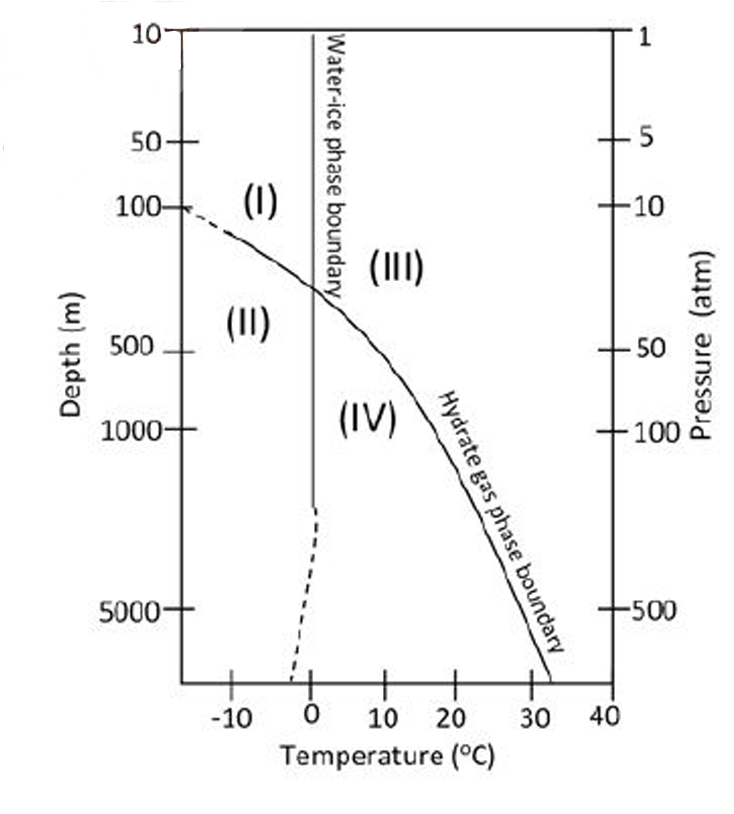
\includegraphics[width=0.5\columnwidth]{Graph_Q55.png}
    \caption{}
    \label{fig:placeholder}
\end{figure}
(P) Methane hydrate + water = gas\\
(Q) Methane gas + water\\
(R) Methane gas + ice\\
(S) Methane hydrate + ice + gas\\

\begin{enumerate}
    \item I-R, II-S, III-P, IV-Q
    \item I-R, II-Q, III-P, IV-S
    \item I-R, II-S, III-Q, IV-P
    \item I-R, II-P, III-S, IV-Q
\end{enumerate}
\hfill{(GATE PE 2017)}

\item The ninth and the tenth of this month are Monday and Tuesday \dots.
\begin{enumerate}
\item figuratively
\item retrospectively
\item respectively
\item rightfully
\end{enumerate}
\hfill{(GATE PE 2017)}

\item It is \dots to read this year's textbook \dots the last year's.
\begin{enumerate}
\item easier, than
\item most easy, than
\item easier, from
\item easiest, from
\end{enumerate}
\hfill{(GATE PE 2017)}

\item A rule states that in order to drink beer, one must be over 18 years old. In a bar, there are 4 people. P is 16 years old, Q is 25 years old, R is drinking milkshake and S is drinking a beer. What must be checked to ensure that the rule is being followed?
\begin{enumerate}
\item Only P's drink
\item Only P's drink and S's age
\item Only S's age
\item Only P's drink, Q's drink and S's age
\end{enumerate}
\hfill{(GATE PE 2017)}

\item Fatima starts from point P, goes North for 3 km, and then East for 4 km to reach point Q. She then turns to face point P and goes 15 km in that direction. She then goes North for 6 km. How far is she from point P, and in which direction should she go to reach point P?
\begin{enumerate}
\item 8 km, East
\item 12 km, North
\item 6 km, East
\item 10 km, North
\end{enumerate}
\hfill{(GATE PE 2017)}

\item 500 students are taking one or more courses out of Chemistry, Physics, and Mathematics. Registration records indicate course enrolment as follows: Chemistry (329), Physics (186), Mathematics (295), Chemistry and Physics (83), Chemistry and Mathematics (217), and Physics and Mathematics (63). How many students are taking all 3 subjects?
\begin{enumerate}
\begin{multicols}{4}
\item 37
\item 43
\item 47
\item 53
\end{multicols}
\end{enumerate}
\hfill{(GATE PE 2017)}


\item ``If you are looking for a history of India, or for an account of the rise and fall of the British Raj, or for the reason of the cleaving of the subcontinent into two mutually antagonistic parts and the effects this mutilation will have in the respective sections, and ultimately on Asia, you will not find it in these pages; for though I have spent a lifetime in the country, I lived too near the seat of events, and was too intimately associated with the actors, to get the perspective needed for the impartial recording of these matters.''\\
Which of the following statements best reflects the author's opinion?
\begin{enumerate}
\item An intimate association does not allow for the necessary perspective.
\item Matters are recorded with an impartial perspective.
\item An intimate association offers an impartial perspective.
\item Actors are typically associated with the impartial recording of matters.
\end{enumerate}
\hfill{(GATE PE 2017)}

\item Each of P, Q, R, S, W, X, Y and Z has been married at most once. X and Y are married and have two children P and Q. Z is the grandfather of the daughter S of P. Further, Z and W are married and are parents of R. Which one of the following must necessarily be FALSE?
\begin{enumerate}
\item X is the mother-in-law of R
\item P and R are not married to each other
\item P is a son of X and Y
\item Q cannot be married to R
\end{enumerate}
\hfill{(GATE PE 2017)}

\item 1200 men and 500 women can build a bridge in 2 weeks. 900 men and 250 women will take 3 weeks to build the same bridge. How many men will be needed to build the bridge in one week?
\begin{enumerate}
\begin{multicols}{4}
\item 3000
\item 3300
\item 3600
\item 3900
\end{multicols}
\end{enumerate}
\hfill{(GATE PE 2017)}

\item The number of 3-digit numbers such that the digit 1 is never to the immediate right of 2 is
\begin{enumerate}
\begin{multicols}{4}
\item 781
\item 791
\item 881
\item 891
\end{multicols}
\end{enumerate}
\hfill{(GATE PE 2017)}

\item A contour line joins locations having the same height above the mean sea level. The following is a contour plot of a geographical region. Contour lines are shown at 25 m intervals in this plot.\\
Which of the following is the steepest path leaving from P?
\begin{figure}[h]
    \centering
    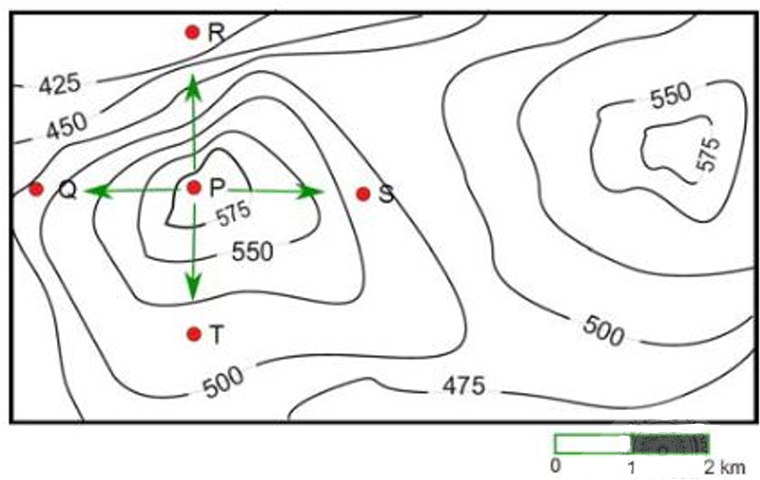
\includegraphics[width=0.5\columnwidth]{Graph_Q65.png}
    \caption{}
    \label{fig:placeholder}
\end{figure}
\begin{enumerate}
\begin{multicols}{4}
    \item P to Q
    \item P to R
    \item P to S
    \item P to T
\end{multicols}
\end{enumerate}
\hfill{(GATE PE 2017)}

\end{enumerate}

\newpage

\begin{tabular}[12pt]{|c|c|c|c|c|}
\hline
Q. No.&Type&Section&Key&Marks  \\
\hline
1&NAT&PE&3.70 to 3.79&1\\
\hline
2&NAT&PE&31.50 to 32.5&1\\
\hline
3&MCQ&PE&D&1\\
\hline
4&MCQ&PE&C&1\\
\hline
5&MCQ&PE&D&1\\
\hline
6&MCQ&B&1\\
\hline
7&MCQ&PE&C&1\\
\hline
8&MCQ&PE&B&1\\
\hline
9&MCQ&PE&B&1\\
\hline
10&NAT&PE&17.00 to 18.00&1\\
\hline
11&MCQ&PE&C&1\\
\hline
12&MCQ&PE&A&1\\
\hline
13&MCQ&B&1\\
\hline
14&MCQ&PE&C&1\\
\hline
15&MCQ&PE&B&1\\
\hline
16&MCQ&PE&D&1\\
\hline
17&MCQ&PE&A&1\\
\hline
18&MCQ&PE&D&1\\
\hline
19&NAT&PE&61.0 to 63.0&1\\
\hline
20&MCQ&PE&A&1\\
\hline
21&MCQ&PE&C&1\\
\hline
22&MCQ&PE&D&1\\
\hline
23&MCQ&PE&D&1\\
\hline
24&MCQ&PE&C&1\\
\hline
25&MCQ&PE&A or D&1\\
\hline
26&NAT&PE&-2.05 to -1.95&2\\
\hline
27&NAT&PE&0.720 to 0.730&2\\
\hline
28&NAT&PE&10.5 to 11.5&2\\
\hline
29&NAT&PE&72.0 to 75.0&2\\
\hline
30&NAT&PE&999.0 to 1001.0&2\\
\hline
31&NAT&PE&1080.0 to 1095.0&2\\
\hline
32&NAT&PE&1990 to 2010&2\\
\hline
33&NAT&PE&7.5 to 8.2&2\\
\hline
34&NAT&PE&14.20 to 14.90&2\\
\hline
35&MCQ&PE&C&2\\
\hline
36&NAT&PE&101.00 to 104.00&2\\
\hline
37&NAT&PE&3.50 to 3.80&2\\
\hline
38&MCQ&PE&C&2\\
\hline
39&NAT&PE&140.0 to 150.0&2\\
\hline
40&MCQ&PE&C&2\\
\hline
41&MCQ&PE&B&2\\
\hline
42&MCQ&PE&B&2\\
\hline
43&MCQ&PE&3D&2\\
\hline
44&NAT&PE&60.0 to 65.0&2\\
\hline
45&NAT&PE&13.5 to 15.5&2\\
\hline
46&MCQ&PE&A&2\\
\hline
47&NAT&PE&25.00 to 28.00&2\\
\hline
\end{tabular}
\newpage
\begin{tabular}{|c|c|c|c|c|}
\hline
Q. No&Type&Section&Key&Marks\\
\hline
48&NAT&PE&38200.0 to 38500.0&2\\
\hline
49&NAT&PE&0.55 to 0.65&2\\
\hline
50&NAT&PE&50.0 to 54.0&2\\
\hline
51&MCQ&PE&C&2\\
\hline
52&MCQ&PE&B&2\\
\hline
53&MCQ&PE&C&2\\
\hline
54&MCQ&PE&A&2\\
\hline
55&MCQ&PE&C&2\\
\hline
56&MCQ&PE&C&1\\
\hline
57&MCQ&PE&A&1\\
\hline
58&MCQ&PE&B&1\\
\hline
59&MCQ&PE&A&1\\
\hline
60&MCQ&PE&D&1\\
\hline
61&MCQ&PE&A&2\\
\hline
62&MCQ&PE&D&2\\
\hline
63&MCQ&PE&C&2\\
\hline
64&MCQ&PE&C&2\\
\hline
65&MCQ&PE&B&2\\
\hline
\end{tabular}

\end{document}



